\documentclass[t, 				             
			   final,
			   12pt, 				         
			   xcolor={usenames,dvipsnames}, 
			   table]{beamer}

% pacotes utilizados.
\usepackage[alf]{abntex2cite}
\usepackage{amsmath}
\usepackage[brazil]{babel}
\usepackage{booktabs}
\usepackage{caption}
\usepackage[utf8]{inputenc}
\usepackage{listings}
\usepackage{multicol}
\usepackage{multirow}
\usepackage{todo}


% configuração do tema
\usetheme[pageofpages=de,
          bullet=square,			
          titleline=true,				
          alternativetitlepage=true,			
          titlepagelogo=imagens/logo-puc,	
          watermarkheight=70px,		
          watermarkheightmult=4	
          ]{Torino}

\setbeamertemplate{sections/subsections in toc}[square]
\setbeamertemplate{bibliography item}[default]

\usecolortheme{freewilly}

% Block Environment
% -------------------------------
\setbeamertemplate {blocks}[default]
\setbeamercolor{block title}{fg=red!0!green!15!blue!85!, bg=red!33!green!37!blue!15!}
\setbeamercolor{block body}{fg=black, bg=red!32!green!33!blue!5}
\setbeamercolor{block title alerted}{fg=white, bg=red!40!black}
\setbeamercolor{block body alerted}{fg=black, bg=red!5!white}
\setbeamercolor{block title example}{fg=white, bg=green!40!black}
\setbeamercolor{block body example}{fg=black, bg=green!5!white}
\setbeamerfont{block title}{size=\scriptsize, series=\bfseries}


\definecolor{javared}{rgb}{0.6,0,0} % for strings
\definecolor{javagreen}{rgb}{0.25,0.5,0.35} % comments
\definecolor{javapurple}{rgb}{0.5,0,0.35} % keywords
\definecolor{javadocblue}{rgb}{0.25,0.35,0.75} % javadoc
 
\lstset{}

\lstdefinestyle{BashInputBasicStyle}{
	language=bash,
	basicstyle=\normalsize\ttfamily,
	columns=fullflexible,
	tabsize=2,
	showstringspaces=false,
	frame=single,
	inputencoding=utf8,
	rulecolor=\color{gray}
}

\lstdefinestyle{BashInputStyle}{
  language=bash,
  basicstyle=\normalsize\ttfamily,
  numbers=left,
  numberstyle=\tiny,
  numbersep=2pt,
  frame=tb,
  columns=fullflexible,
  tabsize=2,
  showstringspaces=false,
  commentstyle=\color{gray},
  inputencoding=utf8,
  rulecolor=\color{gray}
}

\lstdefinestyle{RubyInputStyle}{
    language=ruby,
    basicstyle=\scriptsize\ttfamily,
    keywordstyle=\color{javapurple},
    identifierstyle=\color{black},
    commentstyle=\color{javagreen},
	stringstyle=\color{blue},
    showstringspaces=false,
    numbers=left,
    numberstyle=\color{gray}\tiny,
    tabsize=3,
    extendedchars=\true,
    inputencoding=utf8,
%   frame=single, 
    columns=fixed,
    backgroundcolor=\color{red!32!green!33!blue!5}
}    
%  language=ruby,
%  basicstyle=\normalsize\ttfamily,
%  keywordstyle=\color{OrangeRed},
%  identifierstyle=\color{Turquoise},
%  commentstyle=\color{gray},
%  stringstyle=\color{YellowOrange},
%  numbers=left,
%  numberstyle=\tiny,
%  numbersep=2pt,
%  frame=tb,
%  columns=fullflexible,
%  backgroundcolor=\color{white!80},
%  linewidth=0.9\linewidth,
%  tabsize=2,
%  showstringspaces=false
%  inputencoding=utf8


\lstdefinestyle{JavaInputStyle}{
	language=Java,
	basicstyle=\ttfamily,
	keywordstyle=\color{javapurple}\bfseries,
	stringstyle=\color{javared},
	commentstyle=\color{javagreen},
	morecomment=[s][\color{javadocblue}]{/**}{*/},
	numbers=left,
	numberstyle=\tiny\color{black},
	numbersep=10pt,
	tabsize=2,
	showspaces=false,
	showstringspaces=false,
	frame=tb,
	columns=fullflexible,
	backgroundcolor=\color{white!80},
	linewidth=0.9\linewidth,
	inputencoding=utf8
}

\begin{document}
	\author{Luiz Alberto Ferreira Gomes}
\title{Aplicações Web com Ruby On Rails}
\subtitle{Seminários da Computação}
\institute{Curso de Ciência da Computação}
\date{\today}

	\begin{frame}[plain]
  \titlepage
\end{frame}
	\AtBeginSection[]
{
  \begin{frame}{Agenda}
    \tableofcontents[currentsection]
  \end{frame}
}
  
%	\section{Apresentaço do Curso}

%%-------------------------------------------------------------------------------------- Início
\begin{frame}[fragile,t]{Apresentação do Curso}
  \begin{itemize}
    \item Este curso tem como objetivo explorar o \alert{desenvolvimento de aplicações web} considerando 
      \alert{padrões de projetos} fundamentais e filosofias associadas a \alert{arquiteturas modernas} de aplicações web
      , juntamente com os seus principais componentes.
    \item Ao final deste curso, espera-se que o aluno seja capaz de:
    \begin{itemize}
      \item projetar, desenvolver e publicar uma aplicação web;
      \item entender os principais \alert{componentes} da arquitetura web apps e como eles se interagem;
      \item utilizar a plataforma Ruby on Rails;
      \item compreender melhor as \alert{práticas} modernas de engenharia de software.
    \end{itemize}
  \end{itemize}
\end{frame}
%%-------------------------------------------------------------------------------------- Início
\begin{frame}[fragile,t]{Conteúdo Programático}
    \begin{center}
      \begin{tabular}{| p{2cm} | p{8cm} |}
	\hline
	\textbf{Data} & \textbf{Módulo} \\ \hline
	18/09 & Introdução e Conceituação \\ \hline
	25/09 & Ruby on Rails \\ \hline
	02/10 & Interação com Banco de Dados \\ \hline
	09/10 & A Linguagem de Programação Ruby \\ \hline
	16/10 & A Linguagem de Programação Ruby \\ \hline
	23/10 & Middleware \\ \hline
	30/10 & Interface com o Usuário \\ \hline
	\hline
      \end{tabular}
    \end{center}  
\end{frame}
%	\section{Aplicação Web}
%%-------------------------------------------------------------------------------------- Início

%%-------------------------------------------------------------------------------------- Início
\begin{frame}[allowframebreaks, fragile,t]{Aplicação Web}
  \begin{exampleblock}{Definição(Aplicação Web)}
    Uma \alert{aplicação web} é aquela que acessada pelos usuários por meio de uma \alert{rede de computadores}, utiliza
    um \alert{navegador} (em inglês: \textit{browser}); e consiste de uma coleção de \alert{\textit{scripts}} no cliente e 
    no servidor, páginas \alert{HTML} e outros recursos que podem estar espalhados por vários servidores. Ele é 
    acessada pelos usuários via \alert{um endereço} que faz referência a um servidor web (por exemplo: www.inf.pucpcaldadas.br).
  \end{exampleblock}
  
  \begin{itemize}
    \item Exemplos: webmail, lojas virtuais, homebanking, wikis, blogs e etc.
  \end{itemize}
  
\framebreak

  \begin{itemize}
    \item Há um pouco mais do que isso:
    \begin{itemize}
      \item Rede de Computadores:
      \begin{itemize}
        \item a \alert{Internet}, um sistema global de redes de computadores interconectadas.
        \item utiliza o conjunto de protocolos TCP/IP.
      \end{itemize}
      \item Web (World Wide Web):
      \begin{itemize}
	\item um sistema de documentos (em inglês: \textit{web pages}) \alert{vinculados} que são acessados através 
	  da Internet via protocolo HTTP.
	\item Web pages contêm documentos \alert{hypermedia}: textos, gráficos, imagens, vídeos e outros recursos multimídia, juntamente com \textit{hiperlinks} para outras páginas
	\item \alert{Hiperlinks} formam a \alert{estrutura básica} da Web.
	\item A estrutura da Web é a que a torna \alert{útil} e de \alert{valor}.
      \end{itemize}
    \end{itemize}
    \item \underline{Vantagens}:
    \begin{itemize}
      \item \alert{Conveniência} pela utilização um web browser como cliente. 
      \item \alert{Compatibilidade} inerente entre plataformas.
      \item Habilidade de \alert{atualizar} e \alert{manter} as aplicações web sem instalação e distribuição de software
        em vários clientes em potencial.
      \item \alert{Redução} dos custos de TI.
    \end{itemize}
    \item \alert{Desvantagens}:
    \begin{itemize}
      \item Interfaces com usuário ainda \alert{não são tão boas} quanto as das aplicações tradicionais.
      \item Maior risco de \alert{comprometimento} da \alert{privacidade} e \alert{segurança dos dados}.
      \item Mais \alert{difícil} de \alert{desenvolver} e \alert{depurar} do que uma aplicação tradicional, pois 
        existem mais partes a se considerar.
    \end{itemize}
  \end{itemize}
\end{frame}
%%-------------------------------------------------------------------------------------- Início
%	\section{Apresentaço do Curso}

%%-------------------------------------------------------------------------------------- Início
\begin{frame}[fragile,t]{Apresentação do Curso}
  \begin{itemize}
    \item Este curso tem como objetivo explorar o \alert{desenvolvimento de aplicações web} considerando 
      \alert{padrões de projetos} fundamentais e filosofias associadas a \alert{arquiteturas modernas} de aplicações web
      , juntamente com os seus principais componentes.
    \item Ao final deste curso, espera-se que o aluno seja capaz de:
    \begin{itemize}
      \item projetar, desenvolver e publicar uma aplicação web;
      \item entender os principais \alert{componentes} da arquitetura web apps e como eles se interagem;
      \item utilizar a plataforma Ruby on Rails;
      \item compreender melhor as \alert{práticas} modernas de engenharia de software.
    \end{itemize}
  \end{itemize}
\end{frame}
%%-------------------------------------------------------------------------------------- Início
\begin{frame}[fragile,t]{Conteúdo Programático}
    \begin{center}
      \begin{tabular}{| p{2cm} | p{8cm} |}
	\hline
	\textbf{Data} & \textbf{Módulo} \\ \hline
	18/09 & Introdução e Conceituação \\ \hline
	25/09 & Ruby on Rails \\ \hline
	02/10 & Interação com Banco de Dados \\ \hline
	09/10 & A Linguagem de Programação Ruby \\ \hline
	16/10 & A Linguagem de Programação Ruby \\ \hline
	23/10 & Middleware \\ \hline
	30/10 & Interface com o Usuário \\ \hline
	\hline
      \end{tabular}
    \end{center}  
\end{frame}
%%-------------------------------------------------------------------------------------- Início
\begin{frame}[fragile,t]{Histórico}
  \begin{figure}[h!]
    \centering
    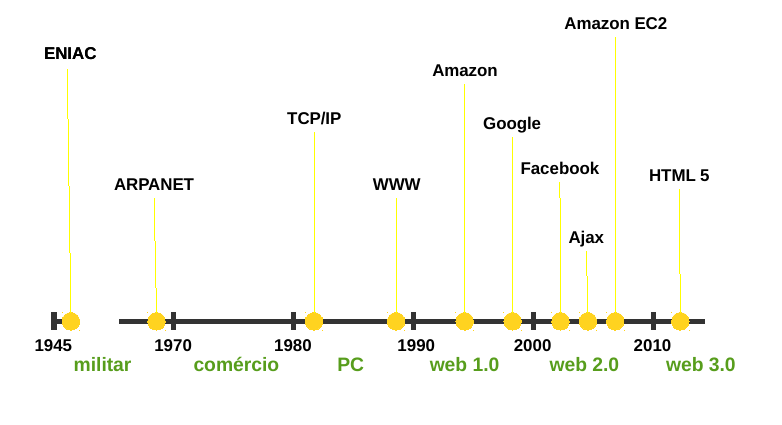
\includegraphics[width=0.95\textwidth]{imagens/historico.png}
  \end{figure} 
\end{frame}
%%-------------------------------------------------------------------------------------- Início
\begin{frame}[fragile,t]{Web 1.0, 2.0 e 3.0}
  \begin{itemize}
    \item \alert{Web 1.0} : páginas estáticas e primeiros modelos de negócios.
    \item \alert{Web 2.0} : interactividade(Ajax), redes sociais e comércio eletrônico.
    \item \alert{Web 3.0} : 'Web Inteligente', interpretação da informação auxiliada por máquina 
    \begin{itemize}
      \item exemplo: sistemas de recomendação.
    \end{itemize}
    \item Base tecnológica da Web 2.0 e 3.0.
    \begin{itemize}
      \item javascript, xml, json(ajax).
      \item interoperabilidade via Web Services.
      \item infraestrutura via modelos de \alert{computação em nuvem} (IAAS, PAAS e SAAS)
      \item aplicações móveis
    \end{itemize}
  \end{itemize}
\end{frame}
%%-------------------------------------------------------------------------------------- Início
\begin{frame}[allowframebreaks, fragile,t]{Modelos de Computação em Nuvem}
  
  \begin{itemize}

    \item \alert{IAAS (Infraestructure As A Service)} : fornece a insfraestrutura computacional
      física ou máquinas virtuais e outros recursos discos, firewalls, endereços IP e etc.
    \begin{itemize}
     \item exemplos: Amazon EC2, Windows Azure, Google Compute Engine.
    \end{itemize}
    
    \item \alert{PAAS (Platform as a Service)} : fornece plataformas computacionais que tipicamente incluem sistemas operacionais,
      ambientes para execução de programas, bancos de dados, servidores web e etc.
    \begin{itemize}
     \item exemplos: AWS Elastic Beanstalk, Windows Azure, Heroku e Google App Engine
    \end{itemize}

    \item \alert{SAAS (Software as a Service)} : fornece acesso sob demanda às aplicações de software, sem que o usuário
      tem que se preocupar com sua instalação, configuração e execução.
    \begin{itemize}
     \item exemplos: Google Apps e Microsoft 365.
    \end{itemize}
 
  \end{itemize}
 
\end{frame}
%	%\section{Arquiteturas de WebApps?}
%%-------------------------------------------------------------------------------------- Início
\begin{frame}[allowframebreaks, fragile,t]{Arquiteturas de Aplicações Web}
  \begin{itemize}
    \item As aplicações \alert{web modernas} envolvem uma quantidade significativa de \alert{complexidade}.
    \begin{itemize}
      \item especialmente no lado do servidor.
    \end{itemize}
    \item Uma típica aplicação web envolve \alert{inúmeros protocolos}, \alert{linguagens de programação} e 
      \alert{tecnologias} que compõem a pilha de tecnologia web. 
    \item Desenvolver, manter e ampliar uma aplicação web complexa é \alert{difícil}.
    \begin{itemize}
      \item mas, construindo-o usando uma \alert{base de princípios de sólidos de projeto} pode-se simplificar 
      cada uma dessas tarefas. 
    \end{itemize}
    \item Engenheiros de software usam \alert{abstrações} para lidar com este tipo de complexidade.
    \begin{itemize}
      \item \textit{Design patterns} fornecem abstrações úteis para sistemas orientados a objetos.
    \end{itemize} 
  \end{itemize}
\end{frame}
%%-------------------------------------------------------------------------------------- Início
\begin{frame}[allowframebreaks, fragile,t]{Design Patterns}
  \begin{exampleblock}{Definição (Design Patterns)}
    Um padrão de projeto é uma descrição da \alert{colaboração de objetos} que interagem para resolver 
    um problema de software em geral dentro de um contexto particular.
  \end{exampleblock}
  \begin{itemize}
    \item Um design pattern é um \alert{modelo abstrato} que pode ser aplicado recorrentemente.
    \item A idéia é aplicar padrões de projeto, a fim de \alert{resolver problemas específicos} que ocorrem 
      durante a construção de sistemas reais.
    \item Os padrões de projeto fornecem uma maneira de \alert{comunicar} as soluções em um projeto, ou seja, 
      é a terminologia que engenheiros de software usam para falar sobre projetos.
  \end{itemize}
\end{frame}
%%-------------------------------------------------------------------------------------- Início
\begin{frame}[allowframebreaks, fragile,t]{Modelo Cliente-Servidor}
	\begin{itemize}
		\item A arquitetura \alert{cliente-servidor} é a arquitetura mais básica para descrever a cooperação
		entre os componentes de uma aplicação web.
		\item A arquitetura cliente-servidor pode ser subdividia em:
		\begin{itemize}
			\item \alert{servidor} que "escuta" por requisições e fornece os serviços ou recursos de acordo com 
			cada  uma.
			\item \alert{cliente} que estabelece a conexão com o servidor para requisitar serviços ou recursos.
		\end{itemize}
		\item Existe um protocolo \alert{request/response} associado com qualquer arquitetura cliente-servidor.
	\end{itemize}
	\begin{figure}[h!]
		\centering
		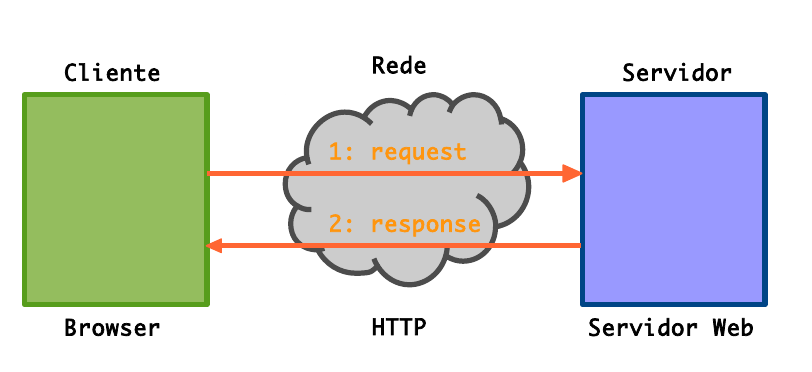
\includegraphics[width=0.90\textwidth]{imagens/cliente-servidor-1.png}
		\caption{Arquitetura cliente servidor.}
	\end{figure} 
	
\framebreak
  \begin{itemize}
    \item É sem dúvida é o padrão de projeto de arquitetura mais conhecido
    \item O ponto chave de uma arquitetura cliente-servidor é \alert{distribuir} os componentes de uma 
      aplicação entre o cliente o servidor de alguma forma. 
    \begin{itemize}
        \item o servidor realiza as tarefas, consultas e transações
        \item o cliente fica com uma responsabilidade menor: a de receber informações
    \end{itemize} 
    \item A fim de construir aplicações web complexas, vários design patterns ajudam a \alert{organizar} como peças 
      são dispostas dentro da arquitetura cliente-servidor.
  \end{itemize}
\end{frame}
%%-------------------------------------------------------------------------------------- Início
\begin{frame}[allowframebreaks, fragile,t]{Arquitetura N-Tier}
  \begin{exampleblock}{Definição (Arquitetura N-Tier)}
    A arquitetura n-tier é um \textit{design pattern} muito útil que estrutura o modelo cliente-servidor.
  \end{exampleblock}
  \begin{itemize}
    \item Este padrão de projeto é baseado no conceito de \alert{quebrar} um sistema em partes diferentes ou 
      camadas que podem ser separados fisicamente:
    \begin{itemize}
      \item cada camada é responsável por fornecer uma \alert{funcionalidade específica} ou coesa. 
      \item uma camada apenas interage com as \alert{camadas adjacentes} a ela por meio de uma 
	\alert{estrutura} bem definida por meio de \alert{interfaces}.
    \end{itemize}
  \end{itemize}
  \begin{exampleblock}{Exemplos (Arquitetura 2-Tier)}
    \begin{itemize}
      \item Servidores de impressão
      \item Aplicações web antigas:
      \begin{itemize}
        \item Interface com o usuário (navegador) residia no cliente (thin). 
        \item Servidor fornecia as páginas estáticas (HTML). 
        \item Interface entre os dois via \textit{Hypertext Transfer Protocol} (HTTP).
      \end{itemize}
    \end{itemize}
  \end{exampleblock}
  \begin{itemize}
    \item Camadas \alert{adicionais} aparecem quando a \alert{funcionalidade} do aplicativo é ainda 
      \alert{mais dividida}.
    \item Quais são as vantagens de um tal projeto? 
    \begin{itemize}
      \item A abstração fornece um meio para \alert{gerenciar} a complexidade. 
      \item Camadas podem ser atualizados ou substituídos de forma \alert{independente} 
	a medida que os requisitos ou tecnologia.
      \begin{itemize}
       \item  a nova só precisa usar as \alert{mesmas interfaces} que a antiga utilizada. 
      \end{itemize}
      \item Ele fornece um \alert{equilíbrio} entre inovação e padronização. 
      \item Sistemas tendem a ser muito mais \alert{fáceis} de construir, manter e atualizar.
    \end{itemize}
  \end{itemize}

\end{frame}
%%-------------------------------------------------------------------------------------- Início
\begin{frame}[allowframebreaks, fragile,t]{Arquitetura 3-Tiers}
  \begin{itemize}
    \item Uma das mais comuns é a arquitetura em 3 camadas: 
    \begin{itemize}
      \item Apresentação
      \begin{itemize}
       \item a interface com o usuário. 
      \end{itemize}     
      \item Aplicação (lógica)
      \begin{itemize}
	\item recupera modifica e$/$ou exclui dados na camada de dados, e envia os resultados do processamento
	para a camada de apresentação. 
      \end{itemize}
      \item Camada de dados
      \begin{itemize}
       \item a fonte dos dados associados ao aplicativo.
      \end{itemize}
    \end{itemize}
 
    \item As aplicações web modernas frequentemente são construídas \alert{utilizando} uma arquitetura em 3 camadas: 
    \begin{itemize}
      \item Apresentação
      \begin{itemize}
	\item o navegador web do usuário. 
      \end{itemize}

      \item Aplicação (lógica) 
      \begin{itemize}     
	\item o servidor web e lógica associada com \alert{geração} de conteúdo web dinâmico.
	\item por exemplo, a coleta e formatação do resultados de uma pesquisa. 
      \end{itemize}
      
      \item Camada de dados
      \begin{itemize}    
	\item um banco de dados.
      \end{itemize}
      
    \end{itemize}
    
  \end{itemize}
\end{frame}
%%-------------------------------------------------------------------------------------- Início
%\begin{frame}[allowframebreaks, fragile,t]{Arquitetura 6-Tiers para Aplicações Web }
%  \begin{itemize}
%    \item A camada de aplicação é frequentemente subdividida em dois níveis:
%    \begin{itemize} 
%      \item Camada de lógica de negócios
%      \begin{itemize}
%	\item modelos os \alert{objetos de negócios} associados ao aplicativo, por exemplo, contas, estoques, etc.
%	\item captura as regras de negócio associadas a esses objetos.     
%       \end{itemize}      
%      \item Camada de acesso a dados
%      \begin{itemize}
%	\item responsável por acessar os dados e passá-los para a camada de lógica de negócios.
%	\item por exemplo, saldos de contas, transações, etc.
%      \end{itemize}
%    \end{itemize}
%    \item A camada de apresentação é muitas vezes subdividida em dois níveis: 
%    \begin{itemize}
%      \item Camada de clientes
%      \begin{itemize}
%	\item os componentes da interface do usuário do lado do cliente.
%      \end{itemize}
%      
%      \item Apresentação camada de lógica
%      \begin{itemize}
%       \item scripts do lado do servidor para a geração de páginas web. 
%      \end{itemize}
%
%    \end{itemize}
%    \item Finalmente, o servidor web é muitas vezes separados em sua própria camada da Web e o
%    servidor de banco de dados na sua camada de dados.
%  \end{itemize}
%  
%  \begin{figure}[h!]
%    \centering
%    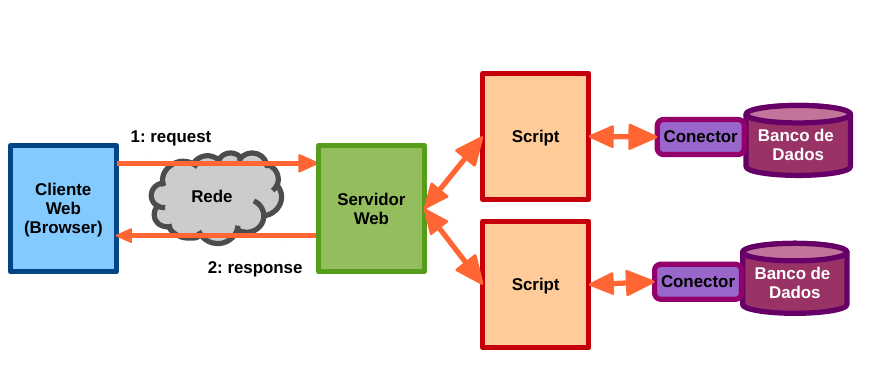
\includegraphics[width=0.95\textwidth]{imagens/cliente-servidor-2.png}
%    \caption{Arquitetura em 6 Camadas.}
%  \end{figure}
%  
%\end{frame}
%%%-------------------------------------------------------------------------------------- Início
	
	\section{Ruby on Rails}
	%-------------------------------------------------------------------------------------- Início
\begin{frame}[fragile, plain, c]{Rails}
	\begin{center}
		\large Rails é um \alert{framework} para construção de \alert{aplicações web} baseado na \alert{linguagem Ruby}.
	\end{center}
\end{frame}
%-------------------------------------------------------------------------------------- Início
\begin{frame}[allowframebreaks, t, fragile]{Rails}
	\begin{itemize}
		\item Rails é fornecido em uma \alert{gem} Ruby (gem é um pacote Ruby)
		\item Rails fornece uma extenso conjunto de geradores de código e scripts de automação de testes
		\item Um conjunto de ferramentas adicionais são fornecidos como parte do ecossistema Rails:
		\begin{itemize}
			\item \alert{Rake} - utilitário similar ao \textbf{make do Unix} para criar e migrar bancos de dados, limpar sessões de uma Web app
			\item \alert{Puma} - servidor web de desenvolvimento para execução de aplicações Rails
			\item \alert{SQLite} - um servidor de banco de dados simples pré-instalado como o Rails
			\item \alert{Rack Middleware} - interface padronizado para interação entre um servidor web e uma Web App
		\end{itemize}
	\end{itemize}
\end{frame}
	
	%%\section{Histórico de Evolução}
%-------------------------------------------------------------------------------------- Início
\begin{frame}[allowframebreaks,fragile,t]{Histórico do Rails}
  \begin{itemize}
    \item David Hanson \alert{derivou} a partir do BaseCamp da 37Signals
    \item 07/2014 - a primeira versão de código aberto liberada
    \item 02/2015 - direitos \alert{colaboração} com o projeto foram liberados
    \item 08/2006 - Apple distribui no Mac OS X "Leopard"
    \item Rails é utilizado pela companhias Airbnb, Disney, GitHub, Shopify e Twitter.
  \end{itemize}

  \begin{figure}[h]
    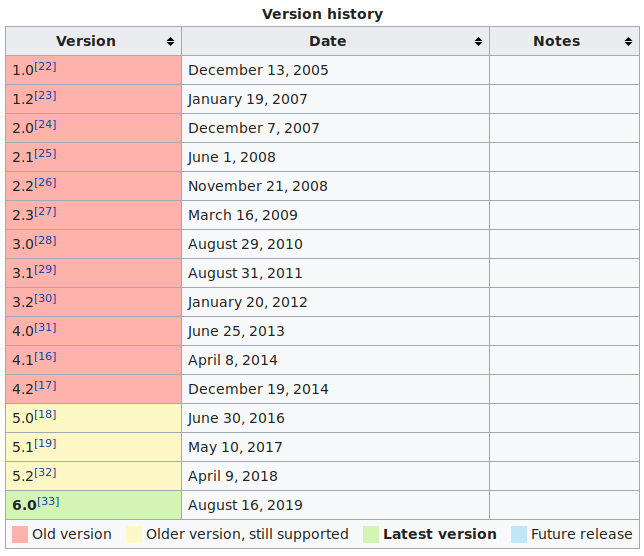
\includegraphics[scale=0.3]{imagens/rails-history.png}  
  \end{figure}
\end{frame}

	\begin{frame}[fragile,t]{Filosofia do Rails}
  \begin{itemize}
    \item Convention Over Configuration (CoC)
    \item Don't Repeat Yourself (DRY)
    \item Representational State Transfer (REST)
  \end{itemize}   
\end{frame}

\begin{frame}[fragile, c]{Convention Over Configuration}
  \begin{center}
    \large se a nomeação \alert{segue} certas \alert{convenções}, não há necessidade de arquivos de \alert{configuração}.
  \end{center}   
\end{frame}

\begin{frame}[fragile, c]{Don't Repeat Yourself}
  \begin{center}
    \large sugere que escrever que o \alert{mesmo código} várias vezes é uma \alert{coisa ruim}
    \end{center}
\end{frame}

\begin{frame}[fragile,t]{Representational State Transfer}
  \begin{center}
    \item organiza a sua aplicação em torno de \alert{recursos} e \alert{padrões} HTTP (verbs)
  \end{center}   
\end{frame}
	%%\section{MVC em Ação no Rails}
%%-------------------------------------------------------------------------------------- Início
\begin{frame}[t, fragile]{Model-View-Controller}
	\begin{itemize}
		\item O framework Rails é contruído em cima do Design Pattern Model View Controller(MVC):
	\end{itemize}
	\begin{figure}[h!]
		\centering
		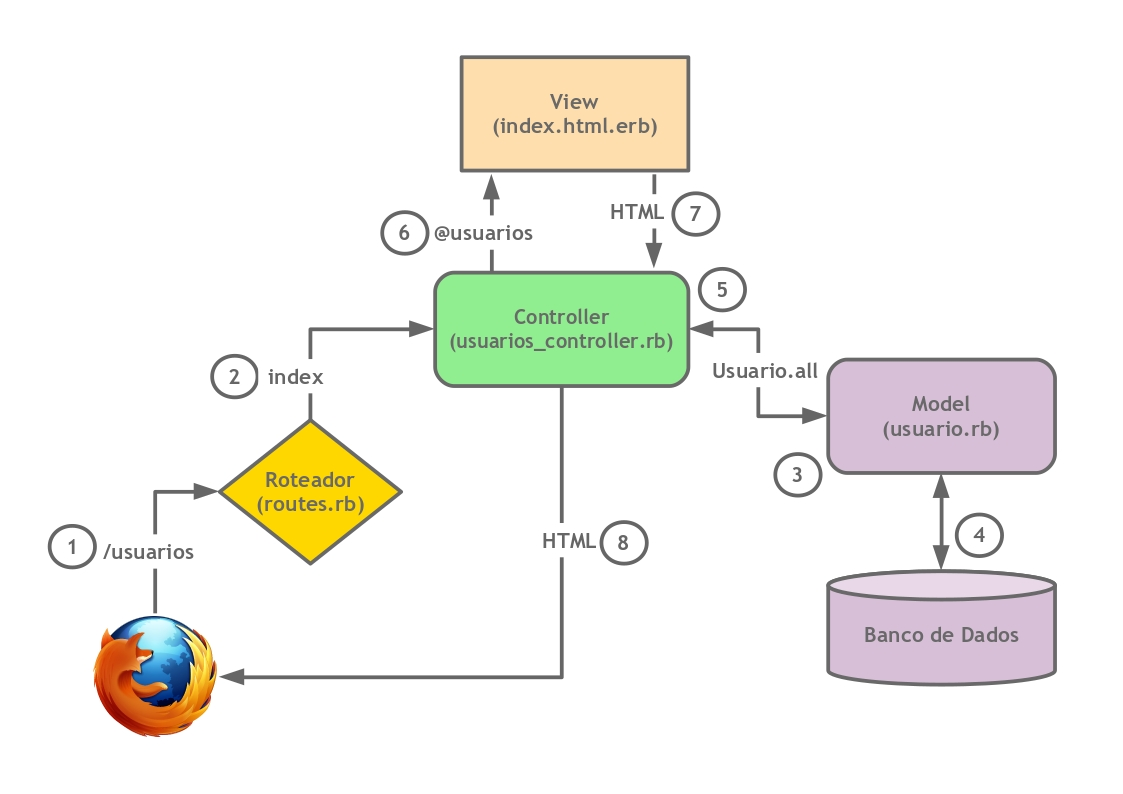
\includegraphics[width=0.70\textwidth]{imagens/mvc.jpg}
	\end{figure}
\end{frame}
 

	%%%-------------------------------------------------------------------------------------- Início
\begin{frame}[fragile,t]{Hora de Colocar a Mão na Massa}
	\begin{itemize}
		\item Conecte-se na máquina com o seu usuário e sua senha
		\begin{enumerate}
	    \item Inicie uma janela de terminal e digite no prompt:
	     \begin{lstlisting}[style=BashInputBasicStyle]
	     $ rails new my_app
	     \end{lstlisting}

	    \item Mude para o diretório da aplicao (RAILS.root)
	     \begin{lstlisting}[style=BashInputBasicStyle]
	     $ cd new my_app
	     \end{lstlisting}
    
	    \item Execute o servidor web embutido:
	    \begin{lstlisting}[style=BashInputBasicStyle]
	    $ rails s
	    \end{lstlisting}
	    
	    \item Abra uma janela do navegador e digite:
	     \begin{lstlisting}[style=BashInputBasicStyle]
	     $ http://localhost:3000
	     \end{lstlisting}
	  \end{enumerate}
	\end{itemize}
\end{frame}

	\include{BlogApp}
	\begin{frame}[fragile,t]{Metodologia de Trabalho}
	\begin{figure}[h!]
		\centering
		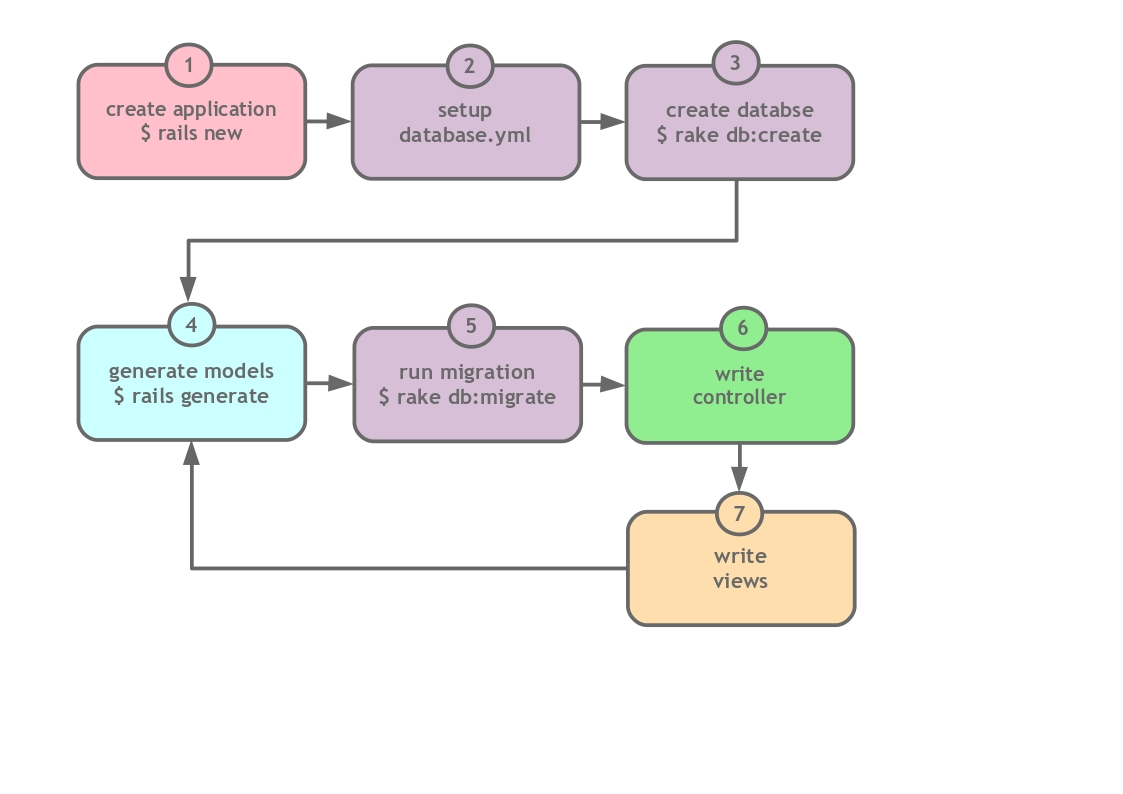
\includegraphics[width=.9\textwidth]{imagens/metodologia-de-trabalho.jpg}
	\end{figure}
\end{frame}

	
%%-------------------------------------------------------------------------------------- Início
%\section{Estrutura de uma Aplicação Rails}
\begin{frame}[allowframebreaks,fragile,t]{Estrutura de uma Aplicação Rails}
  \begin{table}\centering\scriptsize
    \begin{tabular}{@{}lp{8cm}@{}}\toprule
	  \textbf{Arquivo/Pasta} & \textbf{Descrição}	\\ \midrule
	  app & Arquivos contendo os principais códigos da aplicação, incluindo modelos, visões,  
	    controladores e auxiliares(\textit{helpers})\\
	  app/assets & Arquivos contendo folhas de estilos (CSS), códigos Javascript e imagens da 
	    aplicação\\
	  bin & Arquivos ou scripts executáveis\\
	  config & Configurações da aplicação	\\
	  db & Migrações, esquema e outros arquivos relacionados ao banco de dados	\\ 
	  doc & Documentação do sistema	\\
	  lib & Bibliotecas auxiliares	\\
	  lib/assets & Arquivos contendo folhas de estilos (CSS), códigos Javascript e imagens das
	    bibliotecas\\ \bottomrule
    \end{tabular}
  \end{table}	    
  
  \begin{table}\centering\scriptsize
    \begin{tabular}{@{}lp{8cm}@{}}\toprule
      \textbf{Arquivo/Pasta} & \textbf{Descrição}	\\ \midrule
      log & Informações de log	\\
      public & Páginas que podem ser acessadas publicamente via navegador, tais como 
	    páginas de erros	\\    
      test & Testes da nossa aplicação	\\
      tmp & Arquivos temporários como cache e informações de sessões	\\
      vendor & Dependências e bibliotecas de terceiros\\
      vendor/assets & Arquivos contendo folhas de estilos (CSS), códigos Javascript e imagens de
	    terceiros\\
      README.rdoc & Uma breve descrição da aplicação\\
      Rakefile & Tarefas que podem ser executadas pelo comando rake	\\
      Gemfile & Pacotes(gems) necessários para a aplicação	\\
      Gemfile.lock & Uma lista de gems utilizadas para garantir que todas as cópias da aplicação
		      utilizam as mesmas versões de gems\\ 
      config.ru & Um arquivo de configuração para o Rack Middleware\\
      .gitignore & Define de arquivos ou padrões de arquivos que deverão ser ignorados pelo Git\\ \bottomrule
    \end{tabular}
  \end{table} 

\end{frame}	
	\section{Model Component}
\begin{frame}[t, fragile]{Model Component}
	\begin{itemize}
		\item O modelo gerencia os \alert{dados}, a \alert{lógica} e as \alert{regras de negócios} da aplicação.
	\end{itemize}
	\begin{figure}[h!]
		\centering
		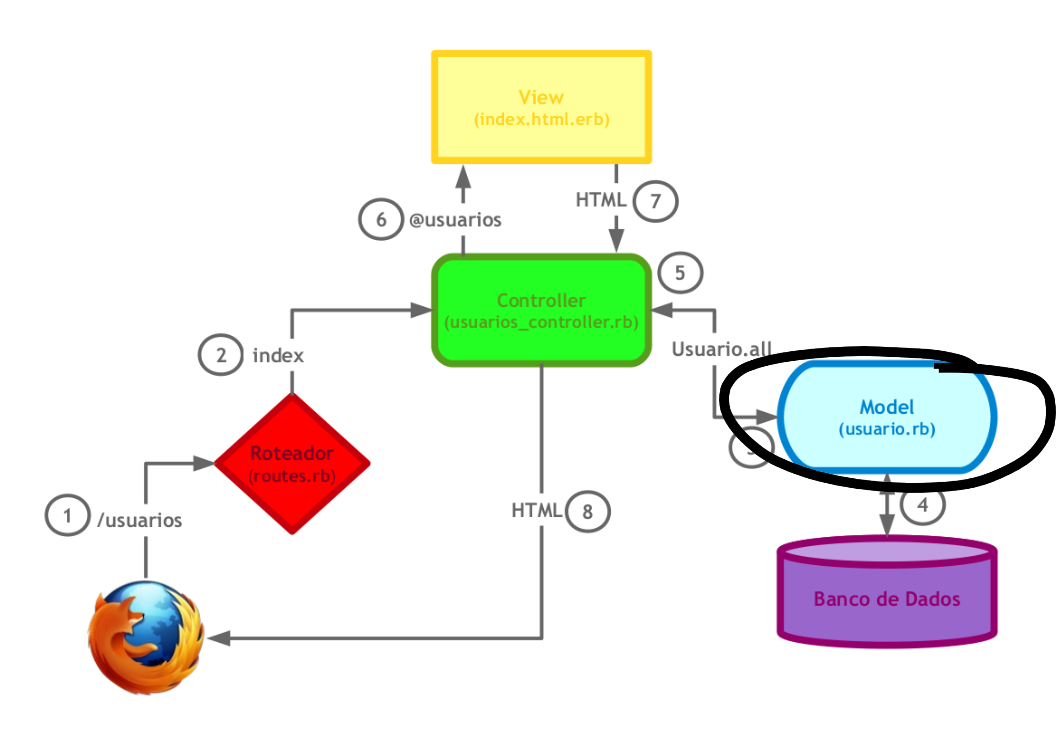
\includegraphics[width=0.75\textwidth]{imagens/mvc-2.png}
	\end{figure}
\end{frame}
	%\section{Banco de Dados Relacionais}
\begin{frame}[t, allowframebreaks, fragile]{Banco de Dados Relacionais}
	\begin{itemize}
		\item Um aspecto importante da programação web é a habilidade de coletar, armazenar e recuperar
		diferentes formas de dados
		\begin{itemize}
			\item uma das formas mais populares são os \alert{bancos de dados relacionais}
		\end{itemize} 
% 		\item maioria banco de dados relacionais acessados através da Structured Query Language (SQL)
		\item Um banco de dados relacional é baseado entidades, denominadas \alert{tabelas}, no
		relacionamento, \alert{associações}, entre elas
		\item O contêiner fundamental em um banco de dados relacional é denominado de \alert{database} ou \alert{schema}
		\begin{itemize}
			\item podem incluir estruturas de dados, os dados propriamente ditos e permissões de acesso
		\end{itemize}  
		\framebreak
		\item Os dados são armazenados em \alert{tabelas} e as tabelas são divididas em \alert{linhas} e \alert{colunas}.
		Por exemplo:
		\begin{table}[tp] 
			\scriptsize 
			\caption{comment}
			\setlength{\tabcolsep}{8pt}
			\setlength{\extrarowheight}{2pt}   			
			\begin{tabular}{|l|l|l|} 
				\hline
				\textbf{id} & \textbf{post\_id} & \textbf{body}\\
				\hline
				10 & 1 & Ruby realmente... \\
				\hline
				11 & 2 & Rails facilita... \\
				\hline
				13 & 2 & Concordo, ... \\
				\hline
			\end{tabular}
		\end{table}
		\pagebreak
		\item Relacionamentos são estabelecidos entre tabelas para que a consistência dos dados
		seja mantida em qualquer situação e podem ser:
		\begin{itemize}
			\item 1:1, 1:N ou N:M
			\begin{columns}[t]
				\column{0.4\textwidth}
				\begin{table}[tp] 
					\scriptsize 
					\caption{comment}
					\setlength{\tabcolsep}{8pt}
					\setlength{\extrarowheight}{2pt}   			
					\begin{tabular}{|l|l|l|} 
						\hline
						\textbf{id} & \textbf{post\_id} & \textbf{body}\\
						\hline
						10 & 1 & Ruby realmente... \\
						\hline
						11 & 2 & Rails facilita... \\
						\hline
						13 & 2 & Concordo, ... \\
						\hline
					\end{tabular}
				\end{table}
				\column{0.6\textwidth}
				\begin{table}[tp] 
					\caption{post}
					\scriptsize 
					\setlength{\tabcolsep}{8pt}
					\setlength{\extrarowheight}{1pt}   			
					\begin{tabular}{|l|l|l|} 
						\hline
						\textbf{id} & \textbf{title} & \textbf{body} \\
						\hline
						\textbf{1} & A Linguagem Ruby & Ruby é legal. \\
						\hline
						\textbf{2} & O Framework Rais & O Rais facilita...\\
						\hline
					\end{tabular}
				\end{table}   		
			\end{columns}
		\end{itemize}  
	\end{itemize}
\end{frame}
	%%-------------------------------------------------------------------------------------- Início
\section{Aplicação Exemplo}
\begin{frame}[allowframebreaks, fragile,t]{Especificação do Blog App}
	\begin{enumerate}
		\item Blog é uma contração de "weblog", um site de discussão ou troca de informações
		publicado na Web.
		\item Existem dois tipos de participantes: o administrador e o usuário
		\item O administrador do blog deve ser capaz de entrar novas postagens, tipicamente
		em ordem cronológica inversa.
		\item Os usuários devem ser capazes de visitar o blog e escrever comentários sobre
		as postagens.
		\item O administrador do blog deve ser capaz de modificar e ou remover qualquer postagem
		ou comentário.
		\item Os usuários não devem ser capazes de modificar postagens ou comentários de outros usuários.
	\end{enumerate}
\end{frame}

\begin{frame}[allowframebreaks, fragile,t]{Passos Iniciais do Blog App}
	\begin{enumerate}
	    \item Inicie uma janela de terminal e digite no prompt:
	     \begin{lstlisting}[style=BashInputBasicStyle]
		     $ cd 
		     $ rails new blog
	     \end{lstlisting}
	    \item Utilize o gerador \verb|scaffold| para criar os 
	    componentes MVC para as postagens e os comentários
	     \begin{lstlisting}[style=BashInputBasicStyle]
		     $ rails generate scaffold post \ 
			     title:string body:text
	     \end{lstlisting}
	    \item Gere as tabelas \verb|post| e \verb|comment| no banco de dados
	    \begin{lstlisting}[style=BashInputBasicStyle]
		    $ rake db:migrate
	    \end{lstlisting}
	    
	    \item Visualize todas as URLs reconhecidas pela sua aplicação digitando:
	    \begin{lstlisting}[style=BashInputBasicStyle]
	    $ rake routes
	    \end{lstlisting}
	     \item Inicie o servidor web embutido:
	     \begin{lstlisting}[style=BashInputBasicStyle]
	     $ rails s
	     \end{lstlisting}
	     
	     \item Abra uma janela do navegador e digite:
	     \begin{lstlisting}[style=BashInputBasicStyle]
	     $ http://localhost:3000/posts
	     \end{lstlisting}
	\end{enumerate}
  
\end{frame}
	\begin{frame}[allowframebreaks, t, fragile]{SQLite}
	\begin{itemize}
		\item O banco de dados que o Rails utiliza em diversos ambientes (desenvolvimento,
		teste e produção) é especificado em: \alert{config/database.yml}
	\end{itemize}
	
	\lstinputlisting[style=RubyInputStyle, firstline=7]{codigos/blog_1/config/database.yml}
	
	\begin{itemize}
		\item Rails usa por padrão o SQLite como gerenciador padrão
		\begin{itemize}
			\item relacional, embutido, sem servidor, configuração zero,
			transacional, suporta SQL
		\end{itemize}
	\end{itemize}
	
	\begin{center}
		\alert{{\huge ATENÇÃO: SQLite não um banco de dados para produção !}}
	\end{center}
	
	\begin{itemize}
		\item Banco de dados de produção populares: \alert{MySQL} e \alert{PostgreSQL}
	\end{itemize}
\end{frame}

\begin{frame}[t, fragile]{Database Console}
	\begin{itemize}
		\item O comando \alert{rails db} fornece uma console para acesso aos bancos dados
		MySQL, PostgreSQL e SQLite.
	\end{itemize}
	
	\begin{lstlisting}[style=BashInputBasicStyle, basicstyle=\tiny\ttfamily,  keepspaces=true]
		$ rails db
		SQLite version 3.8.7.1 2014-10-29 13:59:56
		Enter ".help" for usage hints.
		sqlite> .headers on
		sqlite> .mode columns
		sqlite> select * from posts;
		id          title             body            created_at                  updated_at                
		----------  ----------------  --------------  --------------------------  --------------------------
		5           A Linguagem Ruby  Ruby e legal.  2016-04-30 22:45:20.636363  2016-04-30 22:45:20.636363
		sqlite> 
	\end{lstlisting}
	
	\begin{itemize}
		\item Dica: utilize \alert{headers on} e \alert{mode coluns}
	\end{itemize}
	
\end{frame}

\begin{frame}[allowframebreaks, t, fragile]{Hora de Colocar a Mão na Massa}
	\begin{itemize}
		\item Inicialize \alert{na pasta da aplicação} a console do banco de dados e
		configure a sua exibição:
		\begin{lstlisting}[style=BashInputBasicStyle]
			$ rails db
			sqlite> .headers on
			sqlite> .mode columns
		\end{lstlisting}
		
		\item Exiba os colunas da tabela \verb|posts|:
		\begin{lstlisting}[style=BashInputBasicStyle]
			sqlite> .schema posts
		\end{lstlisting}
		
		\framebreak
		\item Crie um novo \verb|post| e salve no banco de dados:
		\begin{lstlisting}[style=BashInputBasicStyle]
			sqlite> INSERT INTO posts 
			(title, body, created_at, updated_at) 
			VALUES ("Com.pensar 2016", "Tem varios cursos", 
			"2016-05-03 19:50:00", "2016-05-03 19:50:00");
		\end{lstlisting}
		
		\item Exiba todos os \verb|posts|:
		\begin{lstlisting}[style=BashInputBasicStyle]
			sqlite> SELECT * FROM posts;
		\end{lstlisting}
		
		\item Exiba todos os \verb|posts| ordenados pelo título (title):
		\begin{lstlisting}[style=BashInputBasicStyle]
			sqlite> SELECT * FROM posts ORDER BY title;
		\end{lstlisting}
		
		\item Exiba um \verb|post|:
		\begin{lstlisting}[style=BashInputBasicStyle]
			sqlite> SELECT * FROM posts LIMIT 1
		\end{lstlisting}
		
		\item Exiba o \verb|post| cujo \verb|id| é 2:
		\begin{lstlisting}[style=BashInputBasicStyle]
			sqlite> SELECT * FROM posts WHERE id=2;
		\end{lstlisting}
		
		\item Atualize o título \verb|post| cujo o \verb|id| é 2:
		\begin{lstlisting}[style=BashInputBasicStyle]
			sqlite> UPDATE posts SET title="Novo titulo" 
			WHERE id=2;
		\end{lstlisting}
		
		\item Remova \verb|post| cujo o \verb|id| é 2:
		\begin{lstlisting}[style=BashInputBasicStyle]
			sqlite> DELETE FROM posts WHERE id=2;
		\end{lstlisting}
		
	\end{itemize}
\end{frame}
	\begin{frame}[allowframebreaks, t, fragile]{Migrations}
	
		
	\begin{itemize}
		\item \alert{Como podemos rastrear e desfazer alterações em um banco de dados?}
		\item Não existe uma maneira fácil - manualmente é confuso e propenso a erros.
		\item Tipicamente, comandos SQL são dados para criar e modificar tabelas em um
		banco de dados
		\item Mas se houver a necessidade de trocar o banco de dados "durante o voo"?
		\begin{itemize}
		  \item por exemplo, desenvolve-se em SQLite e implanta-se em MySQL.
		\end{itemize}
	\end{itemize}
	
	\begin{center}
		\textcolor{Turquoise}{{\huge SOLUÇÃO: Migrations}}
	\end{center}
	
	\framebreak
	
	\begin{itemize}
		\item A cada vez que o \alert{generate model} é executado na aplicação, o Rails cria um
		arquivo de \alert{migration} de banco de dados. Este arquivo é armazenado em \alert{db/migrate}
		\item Por exemplo: o arquivo \verb|20160430140114_create_posts.rb|
	\end{itemize}
	  
	\lstinputlisting[style=RubyInputStyle]{codigos/blog_1/db/migrate/20160430140114_create_posts.rb}
	
	\begin{itemize}
		\item Rails utiliza o comando \alert{rake} para executar os \alert{migrations} e fazer as alterações
		no banco de dados.
	\end{itemize}
	
	\begin{lstlisting}[style=BashInputBasicStyle]
		$ rake db:migrate
	\end{lstlisting}
	
\end{frame}
	\begin{frame}[allowframebreaks, t, fragile]{Object-Relational Mapping}
	\begin{itemize}
		\item Um ORM \alert{preenche a lacuna} entre banco de dados relacionais e as linguagens de programação
			orientadas a objetos
		\item \alert{Simplifica} bastante a escrita de códigos para acessar o banco de dados.
		\item Tipicamente, comandos SQL são dados para criar e modificar tabelas em um
		banco de dados
		\item No Rails, o Model do MVC utiliza algum framework de ORM
	\end{itemize}	
\end{frame}

\begin{frame}[allowframebreaks, t, fragile]{Active Record}
	\begin{itemize}
		\item ActiveRecord é o nome do \alert{ORM padrão} do Rails?
		\vspace{15pt}
		\begin{columns}[t]
		\column{0.5\textwidth}
			\lstinputlisting[style=RubyInputStyle, caption=app/models/post.rb]{codigos/blog_1/app/models/post.rb}
		\column{0.5\textwidth}   		
			\alert{\Large Onde está código ?}
			\\
			\textcolor{Turquoise}{\Large R: Metaprogramação + Convenção}
		\end{columns}
		
		\item Para que \alert{"mágica"} ocorra:
		\begin{itemize}
			\item o ActiveRecord tem que saber como encontrar o banco de dados (ocorre via \alert{config/database.yml})
			\item \textbf{(Convenção)} existe uma \alert{tabela} com o \alert{nome no plural} da subclasse \verb|ActiveRecord::Base|
			\item \textbf{(Convenção)} espera-se que a tabela tenha uma chave primário denominada \alert{id}
		\end{itemize}
	\end{itemize}
\end{frame}

\begin{frame}[allowframebreaks, t, fragile]{Object-Relational Mapping}
	\begin{itemize}
		\item Um ORM \alert{preenche a lacuna} entre banco de dados relacionais e as linguagens de programação
		orientadas a objetos
		\item \alert{Simplifica} bastante a escrita de códigos para acessar o banco de dados.
		\item Tipicamente, comandos SQL são dados para criar e modificar tabelas em um
		banco de dados
		\item No Rails, o Model do MVC utiliza algum framework de ORM
	\end{itemize}	
\end{frame}

\begin{frame}[allowframebreaks, t, fragile]{Hora de Colocar a Mão na Massa}
	\begin{itemize}
		\item Inicialize \alert{na pasta da aplicação} a console do Rails (não a do banco de dados):
		\begin{lstlisting}[style=BashInputBasicStyle]
			$ rails c
		\end{lstlisting}
		
		\item Exiba os atributos da classe \verb|Post|:
		\begin{lstlisting}[style=BashInputBasicStyle]
			irb(main):004:0> Post.column_names
		\end{lstlisting}
		
		\item Crie um novo \verb|post| e salve no banco de dados:
		\begin{lstlisting}[style=BashInputBasicStyle]
			irb(main):005:0> p1 = Post.new
			irb(main):006:0> p1.title="Temperatura em Pocos"
			irb(main):007:0> p1.body="Esta muito frio..."
			irb(main):008:0> p1.save
		\end{lstlisting}
		
		\item Exiba todos os \verb|posts|:
		\begin{lstlisting}[style=BashInputBasicStyle]
			irb(main):007:0> Post.all
		\end{lstlisting}
		
		\item Exiba todos os \verb|posts| ordenados pelo título (title):
		\begin{lstlisting}[style=BashInputBasicStyle]
			irb(main):007:0> Post.all.order(title: :asc)
		\end{lstlisting}
		
		\item Exiba um \verb|post|:
		\begin{lstlisting}[style=BashInputBasicStyle]
			irb(main):007:0> Post.first
		\end{lstlisting}
		
		\item Exiba o \verb|post| cujo \verb|id| é 2:
		\begin{lstlisting}[style=BashInputBasicStyle]
			irb(main):007:0> Post.find_by(id: 2)
		\end{lstlisting}
		
		\item Atualize o título do primeiro \verb|post|:
		\begin{lstlisting}[style=BashInputBasicStyle]
			irb(main):007:0> p1=Post.first
			irb(main):008:0> p1.update(title: "um novo titulo")
		\end{lstlisting}
		
		\item Remova do primeiro \verb|post|:
		\begin{lstlisting}[style=BashInputBasicStyle]
			irb(main):007:0> p1=Post.first
			irb(main):008:0> p1.destroy
		\end{lstlisting}
		
	\end{itemize}
\end{frame}
	%%-------------------------------------------------------------------------------------- Início
\begin{frame}[t, fragile]{Validação em Aplicações Web}
	\begin{itemize}
		\item \alert{Validação de Dados} é o processo para \alert{garantir} que a aplicação web 
		operem \alert{corretamente}. Exemplo:
		\begin{itemize}
			\item garantir a validação do e-mail, número do telefone e etc
			\item garantir que as "regras de negócios" sejam validadas
		\end{itemize}

		\item A \alert{vulnerabilidade} mais comum em aplicação web é a \alert{injeção} SQL
	\end{itemize}	
\end{frame}
%%-------------------------------------------------------------------------------------- Início
\begin{frame}[t, fragile]{Client Side}
	\begin{itemize}
		\item Envolve a verificação de que os formulários HTML sejam preechidos corretamente
		\begin{itemize}
			\item \alert{JavaScript} tem sido tradicionalmente utilizado.
			\item \alert{HTML5} possui "input type" específicos para checagem.
			\item Funciona melhor quando combinada com validações do lado do servidor.
		\end{itemize}
	\end{itemize}
\end{frame}
%%-------------------------------------------------------------------------------------- Início
\begin{frame}[t, fragile]{Server Side}
	\begin{itemize}
		\item A validação é feita após a submissão do formulário HTML
		\begin{itemize}
			\item \alert{banco de dados}(stored procedure) - dependente do banco de dados
			\item \alert{no controlador} - veremos mais tarde que não se pode colocar muita lógica no controlador (controladores magros)
			\item \alert{no modelo} - boa maneira de garantir que dados válidos sejam armazenados
				no banco de dados (database agnostic)
			\item Funciona melhor quando combinada com validações do lado do servidor.
		\end{itemize}
	\end{itemize}	
\end{frame}
%%-------------------------------------------------------------------------------------- Início
\begin{frame}[allowframebreaks, t, fragile]{Validação em Rails}
	\begin{itemize}
		\item \alert{Objetos} em um sistema OO como tendo um \alert{ciclo de vida}
		\begin{itemize}
			\item eles são criaddos, atualizados mais tarde e também destruidos.
		\end{itemize}
				
		\item Objetos ActiveRecord têm \alert{métodos} que podem ser chamados, a fim de
		assegurar a sua \alert{integridade} nas várias fases do seu ciclo de vida.
		\begin{itemize}
			\item garantir que todos os atributos são \alert{válidos} antes de salvá-lo no
				banco de dados
		\end{itemize}
		
		\item \alert{Callbacks} são métodos que são invocados em um ponto do ciclo 
			de vida dos objetos ActiveRecord
		\begin{itemize}
			\item eles são "ganchos" para gatilhos para acionar uma lógica quando houver
			alterações de seus objetos
		\end{itemize}
	\end{itemize}
\end{frame}
%%-------------------------------------------------------------------------------------- Início
\begin{frame}[t, fragile]{Validação em Rails}
	\begin{itemize}
		\item \alert{Validations} são tipo de \alert{callbacks} que podem ser utilizados 
			para garantir a validade do dado em um banco de dados 
		
		\item Validação são definidos nos \alert{modelos}. Exemplo:
		\begin{lstlisting}[style=RubyInputStyle]
class Person < ApplicationRecord 
    validates_presence_of :name
    validates_numeracality_of :age, :only_integer => true 
    validates_confirmation_of :email
    validates_length_of :password, :in => 8..20	
end 
		\end{lstlisting}			
		
	\end{itemize}
\end{frame}
	\begin{frame}[allowframebreaks, t, fragile]{I2 - Hora de Colocar a Mão na Massa}
	\begin{itemize}
			
		\item Modifique o arquivo \verb|app/models/post.rb| para exigir 
			que o usuário digite o título e o texto do blog:
		\begin{lstlisting}[style=RubyInputStyle]
			class Post < ApplicationRecord
			  validates_presence_of :title, :body
			end
		\end{lstlisting}
		
		\item Modifique o arquivo \verb|app/models/comment.rb| para exigir 
		que o usuário digite texto do comentário blog:
		\begin{lstlisting}[style=RubyInputStyle]
			class Comment < ApplicationRecord
		    validates_presence_of :body
			end
		\end{lstlisting}
		
		\item Inclua as seguintes instruções no início do arquivo \verb|_form.html.rb| para
		 mostrar as mensagens de validação:
		\begin{lstlisting}[style=RubyInputStyle, caption=app/views/posts/\_form.html.erb]
<% if @post.errors.any? %>
  <div class="alert alert-danger" role="alert">
    <h4 class="alert-heading">Request failed!</h4>
    <ul>
      <% @post.errors.full_messages.each do |message| %>
        <li><%= message %></li>
      <% end %>
    </ul>
    <hr>
    <p class="mb-0">Please, correct issues and try again.</p>
  </div>
<% end %>

		\end{lstlisting}
		
%		\item \alert{Reinicie} a console do Rails tente criar um Post e um Comment
%\begin{lstlisting}[style=BashInputBasicStyle]
%		irb(main):005:0> p1 = Post.new
%		irb(main):006:0> p1.body="Tem algo errado..."
%		irb(main):007:0> p1.save
%		irb(main):008:0> Post.all
%		irb(main):009:0> c1 = Comment.new
%		irb(main):010:0> c1.save
%		irb(main):011:0> Comment.all
%end{lstlisting}	
	\end{itemize}
\end{frame}
	%%-------------------------------------------------------------------------------------- Início
\begin{frame}[allowframebreaks, t, fragile]{Associações em Rails}
	\begin{itemize}
		\item O gerador de modelos utiliza por padrão o ActiveRecord. Isto significa:
		\begin{itemize}
			\item Tabelas para postagens e comentários foram criadas quando executamos as migrações
			\item Um conexão com o banco de dados é estabelecida
			\item O ORM é configurado para as postagens e comentátios foi criado - o "M" do
			MVC.
		\end{itemize}

		\item No entanto, uma coisa está faltando:
		\begin{itemize}
			\item  \alert{tem-se que assegurar que qualquer
				comentários sejam associados às suas postagens}
		\end{itemize}

		\item Para tornar os modelos em Rails totalmente funcionais precisamos adicionar
		\alert{associações}:
		\begin{itemize}
			\item cada postagem precisa saber os comentários associado a ele
			\item cada comentário precisa saber qual é a postagem ele pertence
		\end{itemize}
	
		\item Há uma relação \alert{muitos-para-um} entre comentários e postagens
		uma:
		\begin{figure}[h!]
			\centering
			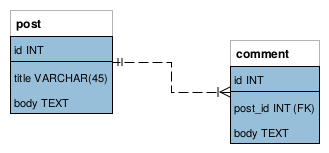
\includegraphics[width=0.70\textwidth]{imagens/modelo-de-dados-blog.png}
		\end{figure}
		
		\item O ActiveRecord contém um conjunto de métodos de classe para
		\alert{vinculação} de objetos por meio de \alert{chaves estrangeiras}
		
		\item Para habilitar isto, deve-se declarar as \alert{associações} dentro dos modelos
		usando:
		\begin{table}[tp] 
			\scriptsize 
			\setlength{\tabcolsep}{8pt}
			\setlength{\extrarowheight}{2pt}   			
			\begin{tabular}{|l|l|l|} 
				\hline
				\textbf{Associação} & \textbf{Modelo Pai} & \textbf{Modelo Filho}\\
				\hline
				Um-para-um & \verb|has_one| & \verb|belongs_to| \\
				\hline
				Muitos-para-um & \verb|has_many| & \verb|belongs_to| \\
				\hline
				Muitos-para-muitos & \verb|has_and_belongs_to_many| & *na tabela junção \\
				\hline
			\end{tabular}
		\end{table}
		
	\end{itemize}	
\end{frame}
	\begin{frame}[allowframebreaks, t, fragile]{I3 - Hora de Colocar a Mão na Massa}
	\begin{itemize}
		\item Modifique o arquivo \verb|app/models/post.rb| para associar 
		o post aos seus comentário:
		\begin{lstlisting}[style=RubyInputStyle]
			class Post < ApplicationRecord
			  validates_presence_of :title, :body
			  has_many :comments
			end
		\end{lstlisting}
		
		\item Modifique o arquivo \verb|app/models/comment.rb| para associar 
		o comentário ao seu post:
		\begin{lstlisting}[style=RubyInputStyle]
			class Comment < ApplicationRecord
			  validates_presence_of :body
			  belongs_to :post
			end
		\end{lstlisting}
		
%		\item Crie um novo \verb|post| e salve no banco de dados (\alert{Reinicie a console do Rails}):
%		\begin{lstlisting}[style=BashInputBasicStyle]
%			irb(main):005:0> p1 = Post.new
%			irb(main):006:0> p1.title="Associacao"
%			irb(main):007:0> p1.body="Eu tenho comentarios!"
%			irb(main):008:0> p1.save
%		\end{lstlisting}
		
%		\item Crie um novo \verb|comment| e o vincule a um \verb|post|:
%		\begin{lstlisting}[style=BashInputBasicStyle]
%			irb(main):005:0> c1 = Comment.new
%			irb(main):006:0> c1.body="Eu sou de um post!"
%			irb(main):007:0> c1.post = p1
%			irb(main):008:0> c1.save
%		\end{lstlisting}
		
%		\item Consulte os comentários do \verb|post| p1:
%		\begin{lstlisting}[style=BashInputBasicStyle]
%			irb(main):005:0> p1.comments.all
%		\end{lstlisting}
		
%		\item Consulte os comentários 2 do \verb|post| p1:
%		\begin{lstlisting}[style=BashInputBasicStyle]
%			irb(main):005:0> p1.comments.where(id: 2)
%		\end{lstlisting}
		
%		\item Consulte o \verb|post| do comentário c1:
%		\begin{lstlisting}[style=BashInputBasicStyle]
%			irb(main):005:0> c1.post
%		\end{lstlisting}
					
	\end{itemize}
\end{frame}
	%%-------------------------------------------------------------------------------------- Início
\section{Controlador}
\begin{frame}[allowframebreaks, t, fragile]{Controlador}
	\begin{itemize}
		\item Um \alert{Action Controller} é classe Ruby contendo uma ou mais ações
		\item Cada \alert{ação} é responsável pela resposta a uma requisição
		\item Quando uma ação é concluída a \alert{visão} de mesmo nome é \alert{renderizada}
		\item Uma ação deve estar \alert{mapeada} no arquivo \alert{routes.rb}:
	\end{itemize}	
	\begin{figure}[h!]
		\centering
		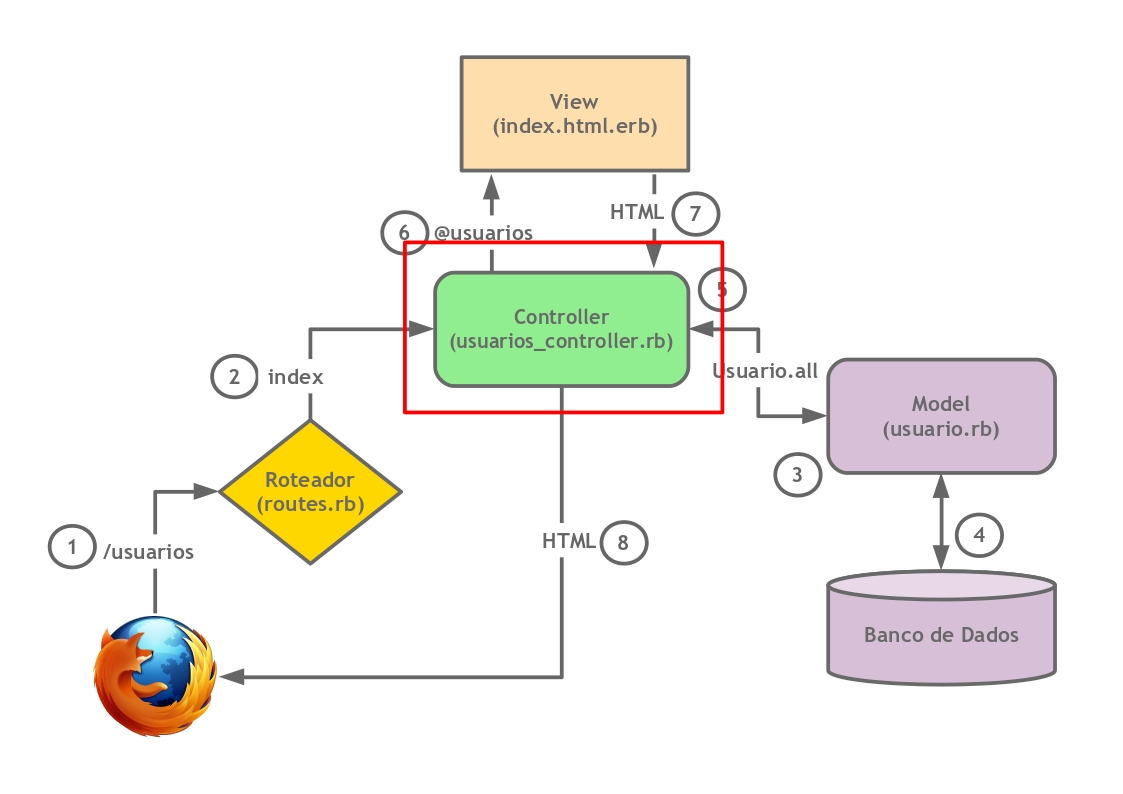
\includegraphics[width=0.80\textwidth]{imagens/mvc-controller.jpg}
	\end{figure}

\end{frame}
	%%-------------------------------------------------------------------------------------- Início
\begin{frame}[allowframebreaks, t, fragile]{Representational State Transfer}
	\begin{itemize}
		\item Representational State Transfer(REST) = Resources
		\item Uma aplicação deverá ser capaz de:
		\begin{itemize}
			\item \alert{List} todos os recursos disponíveis
			\item \alert{Show} um recurso específico
			\item \alert{Destroy} um recurso existente
			\item \alert{Provide a way to create} um novo recurso
			\item \alert{Create} um novo recurso
			\item \alert{Provide a way to update} um recurso existente
			\item \alert{Update} um recurso existente
		\end{itemize}		
	\end{itemize}	
\end{frame}	
	\begin{frame}[allowframebreaks, t, fragile]{I4 - Hora de Colocar a Mão na Massa}
	\begin{itemize}
		
		\item Inicie o servidor web
		\begin{lstlisting}[style=BashInputBasicStyle]
			$ rails s
		\end{lstlisting}
		
		\item Acesse a url \url{http:\\localhost:3000/posts}. Veja o erro que ocorreu.
		
		\item Gere o controlador para os posts:
		\begin{lstlisting}[style=BashInputBasicStyle]
			$ rails generate controller posts
		\end{lstlisting}
		
		\item Reinicie o servidor web e acesse a url \url{http:\\localhost:3000/posts}. Veja o erro que ocorreu.
		
		\item Modifique o arquivo \verb|config/routes.rb| para acrescentar a rota para
		os posts:
		\begin{lstlisting}[style=RubyInputStyle]
			Rails.application.routes.draw do 
				resource :posts
			end 
		\end{lstlisting}	
		
		\item Execute o comando \verb!rake! para visualizar as rotas para os
		posts:
		\begin{lstlisting}[style=BashInputBasicStyle]
			$ rake routes
		\end{lstlisting}
		
		\item Reinicie o servidor web e acesse a url \url{http:\\localhost:3000/posts}. Veja o erro que ocorreu.

	\end{itemize}
\end{frame}
	%%-------------------------------------------------------------------------------------- Início
\begin{frame}[allowframebreaks, t, fragile]{Ação: Index}
	\begin{itemize}
		\item Ação que recupera \alert{todas as postagens} do blog
		\item (Implicitamente) procura pelo template \alert{index.html.erb} para renderizar a resposta
		\begin{lstlisting}[style=RubyInputStyle, caption=controllers/posts\_controller.rb]
Class PostsController < ApplicationController
	def index
		@posts = Post.all
	end
end 
		\end{lstlisting}		
		\framebreak
		\item \alert{index.html.erb}:
		\begin{lstlisting}[style=RubyInputStyle, caption=views/posts/index.html.erb]
<p id="notice"><%= notice %></p>
<h1>Posts</h1>
<table>
  <thead>
    <tr>
      <th>Titulo</th>
      <th>Conteudo</th>
      <th colspan="3"></th>
    </tr>
  </thead>

  <tbody>
  <% @posts.each do |post| %>
    <tr>
      <td><%= post.title %></td>
      <td><%= post.body  %></td>
      <td><%= link_to 'Show', post %></td>
      <td><%= link_to 'Edit', 
      	edit_post_path(post) %></td>
      <td><%= link_to 'Delete', post, method: :delete, 
        data: { confirm: 'Tem certeza ?' } %></td>
    </tr>
  <% end %>
  </tbody>
</table>	
<%= link_to 'New Post', new_post_path %>	
\end{lstlisting}
	\end{itemize}	
\end{frame}
	\begin{frame}[t, fragile]{I5 - Hora de Colocar a Mão na Massa}
	\begin{itemize}
		\item Implemente a ação \alert{index} no controlador de posts e a visão correspondente conforme os slides anteriores
		\item Reinicie o servidor web e acesse a url \url{http:\\localhost:3000/posts}. 
	\end{itemize}
\end{frame}
  %%-------------------------------------------------------------------------------------- Início
\begin{frame}[allowframebreaks, t, fragile]{Ação: Show}
	\begin{itemize}
		\item Recupera \alert{uma} postagem específica no parâmetro \alert{id} passado como parte da URL
		\item (Implicitamente) procura pelo \alert{show.html.erb} para renderizar a resposta
		\begin{lstlisting}[style=RubyInputStyle, caption=controllers/posts\_controller.rb]
Class PostsController < ApplicationController
	before_action :set_post, only: [:show, :edit, 
		:update, :destroy]
	
	def show 
	end 
	
	private
		def set_post 
			@post = Post.find(params[:id])
		end 
		\end{lstlisting}		
		\framebreak
		\item \alert{show.html.erb}:
		\begin{lstlisting}[style=RubyInputStyle, caption=views/posts/show.html.erb]
<p>
	<strong>Title:</strong>
	<%= @post.title %>
</p>
<p>
<strong>Body:</strong>
	<%= @post.body %>
</p>
<%= link_to 'Edit', edit_post_path(@post) %> |
<%= link_to 'Back', posts_path %>	
		\end{lstlisting}		
	\end{itemize}	
\end{frame}
  \begin{frame}[t, fragile]{I6 - Hora de Colocar a Mão na Massa}
	\begin{itemize}
		
		\item Implemente a ação \alert{show} no controlador de posts e a visão correspondente conforme os slides anteriores
		\item Reinicie o servidor web e acesse a url \url{http:\\localhost:3000/posts} e clique em \alert{"Show"}.
	\end{itemize}
\end{frame}
	%%%-------------------------------------------------------------------------------------- Início
\begin{frame}[allowframebreaks, t, fragile]{respond\_to}
	\begin{itemize}
		\item Rails \alert{helper} que \alert{especifica como responder a uma requisição} baseado no 
			formato da requisição
	\end{itemize}	
	\begin{lstlisting}[style=RubyInputStyle, caption=controllers/posts\_controller.rb]
Class PostsController < ApplicationController

  # POST /posts
  # POST /posts.json
  def create
    @post = Post.new(post_params)

    respond_to do |format|
      if @post.save
        format.html { redirect_to @post, notice: 'Post was successfully created.' }
        format.json { render :show, status: :created, location: @post }
      else
        format.html { render :new }
        format.json { render json: @post.errors, status: :unprocessable_entity }
      end
    end
  end
	\end{lstlisting}	
\end{frame}
	%%%-------------------------------------------------------------------------------------- Início
\begin{frame}[allowframebreaks, t, fragile]{redirect_to}
	\begin{itemize}
		\item Ao invés de renderizar um template - \alert{envia uma resposta} ao navegador:
			"go here" 
		\item Usualmente \alert{utiliza uma URL completa} como um parâmetro
		\begin{itemize}	
			\item \item pode ser tanto uma URL ou uma rota nomeada
		\end{itemize}	
		\item Se o parâmetro é um objeto - Rails tentara \alert{gerar uma URL} para aquele objeto
	\end{itemize}	
\end{frame}
	%%-------------------------------------------------------------------------------------- Início
\begin{frame}[allowframebreaks, t, fragile]{Ação: Destroy}
	\begin{itemize}
		\item Recupera uma postagem específica no parâmetro \alert{id} passado como parte da URL
		\item (Implicitamente) procura pelo \alert{show.html.erb} para renderizar a resposta
		\begin{lstlisting}[style=RubyInputStyle, caption=posts_controller.rb]
			Class PostsController < ApplicationController
				before_action :set_post, only: [:show, :edit, :update, :destroy]
				
				#DELETE /posts/1
				#DELETE /posts/1.json 
				def destroy
					@post.destroy
					respond_to do |format|
						format.html {redirect_to posts_url, notice: 'Post was successfully destroyed.'} 
						format.json {head :no_content}
					end
				end 
				
				private
					# Use callbacks to share common setup or constraints between actions.
					def set_post 
						@post = Post.find(params[:id])
					end 
		\end{lstlisting}		
	\end{itemize}	
\end{frame}
  \begin{frame}[t, fragile]{I7 - Hora de Colocar a Mão na Massa}
	\begin{itemize}
		
		\item Implemente a ação \alert{destroy} no controlador de posts e a visão correspondente conforme os slides anteriores
		\item Reinicie o servidor web e acesse a url \url{http:\\localhost:3000/posts} e clique em \alert{"Remove"}.
	\end{itemize}
\end{frame}	
	%%-------------------------------------------------------------------------------------- Início
\begin{frame}[allowframebreaks, t, fragile]{Partials}
	\begin{itemize}
		\item Rails encoraja o princípio DRY	
		\item O laioute da aplicação é mantida em um único local no arquivo \alert{application.html.erb}
		\item O código comum dos templates ser reutilizado em \alert{múltiplos templates}
		\item Por exemplo, os formulários do \alert{edit} e do \alert{new} - são realmente muito diferentes ?
		\item Partials são similares aos templates regulares, mas ele possuem capacidades mais \alert{refinadas}
		\item Nomes de partials começam com \alert{underscore} (\_) 
		\item Partials são renderizados com \alert{render 'partialname'} (sem underscore)
		\item \alert{render} também aceita um segundo argumento, um hash com as variáveis locais utilizadas no partial
		\item Similar a passagem de variáveis locais, o \alert{render} pode receber um objeto
		\item \alert{<%= render @post %>} renderizara \alert{app/views/posts/_posts.html.erb} com o conteúdo da variavel @post
		\item \alert{<%= render @posts %>} renderiza uma coleção e é equivalente a:
		\begin{lstlisting}[style=RubyInputStyle, caption=posts_controller.rb]
			<% @posts.each do |posts	| %> 
				<%= render post %>
			<% end %>
		\end{lstlisting}		
		\begin{itemize}
			\item \alert{_form.html.erb}
		\end{itemize}
				
	\end{itemize}	
\end{frame}



	\begin{frame}[t, fragile]{I8 - Hora de Colocar a Mão na Massa}
	\begin{itemize}		
		\item Implemente o partials \alert{\_form.html.erb} na pasta \alert{view/posts}
	\end{itemize}
\end{frame}
	%%-------------------------------------------------------------------------------------- Início
\begin{frame}[allowframebreaks, t, fragile]{Ação: New}
	\begin{itemize}
		\item Cria um novo objeto \alert{post}(vazio) 
		\item (Implicitamente) procura pelo \alert{new.html.erb} para renderizar a resposta
		\begin{lstlisting}[style=RubyInputStyle, caption=posts_controller.rb]
			Class PostsController < ApplicationController
				
				#GET /posts/new  
				def new
					@post = Post.new 
				end 
				
		\end{lstlisting}		
		
		\item \alert{new.html.erb}:
		
				
	\end{itemize}	
\end{frame}
	\begin{frame}[t, fragile]{I11 - Hora de Colocar a Mão na Massa}
	\begin{itemize}
		\item Implemente a ação \alert{new} no controlador de posts e a visão correspondente conforme os slides anteriores
		\item Reinicie o servidor web e acesse a url \url{http:\\localhost:3000/posts} e clique em \alert{"New Post"}.
	\end{itemize}
\end{frame}	
	%%-------------------------------------------------------------------------------------- Início
\begin{frame}[allowframebreaks, t, fragile]{Ação: Create}
	\begin{itemize}
		\item Cria um novo objeto \alert{post} como os parâmetros que foram passados pelo 
			formulário \alert{new}
		\item Tentar \alert{salvar} o objeto no \alert{banco de dados}
		\item Se sucesso, redireciona para o template \alert{show}
		\item Se insucesso, renderiza o template \alert{new} novamente
		\begin{lstlisting}[style=RubyInputStyle, caption=posts_controller.rb]
			Class PostsController < ApplicationController
			  #POST /posts
			  #POST /posts.json 
			  def create
			    ....
			  end 
				
			  private 
			    # Never trust parameters from the scary internet, only allow the white list through.
			    def post_params 
			    	params.require(:post).permite(:title, :content)
			    end 
				
		\end{lstlisting}		
		\begin{itemize}
			\item a linha .. implementa \alert{strong parameters}
		\end{itemize}
				
	\end{itemize}	
\end{frame}

%%-------------------------------------------------------------------------------------- Início
\begin{frame}[t, fragile]{Hora de Colocar a Mão na Massa}
	\begin{itemize}
		\item Modifique o post_params para o código abaixo:
		\begin{lstlisting}[style=RubyInputStyle, caption=posts_controller.rb]
			Class PostsController < ApplicationController
			  private 
			    # Never trust parameters from the scary internet, only allow the white list through.
			    def post_params 
			    	#params.require(:post).permite(:title, :content)
			    	parmas
			    end 
		\end{lstlisting}		
		\begin{itemize}
			\item tente, agora, criar um post (volte agora para o código original).
		\end{itemize}
				
	\end{itemize}	
\end{frame}


	\begin{frame}[t, fragile]{I10 - Hora de Colocar a Mão na Massa}
	\begin{itemize}
		\item Implemente a ação \alert{create} no controlador de posts
		\item Reinicie o servidor web e acesse a url \url{http:\\localhost:3000/posts}, clique em \alert{"New Post"} e em \alert{"Create Post"}.
	\end{itemize}
\end{frame}	
	%%-------------------------------------------------------------------------------------- Início
\begin{frame}[allowframebreaks, t, fragile]{Flash}
	\begin{itemize}
		\item \textbf{\alert{Problema:}} Queremos \alert{redirecionar} um usuário para uma página 
			diferente do nosso site, mas ao mesmo tempo \alert{fornecer} a ele algum tipo de mensagem.
			Exemplo: "Postagem criada !" 
		\item \textbf{\alert{Solução:}} flash - uma \alert{hash} onde a dado persiste por exatamente 
			\alert{UMA requisição APÓS} a requisição corrente
		\item Um conteúdo pode ser colocado em um flash assim:
		\begin{lstlisting}[style=RubyInputStyle, caption=controllers/posts\_controller.rb] 
			flash[:attribute] = value
		\end{lstlisting}		
		\item Dois atributos \alert{comuns} são \alert{:notice}(\textcolor{Green}{good}) e \alert{:alert}
			(\alert{bad})
		\item Estes dois atributos (:notice ou :alert) podem ser colocados no redirect\_to
		\item \alert{show.html.erb}:
		\begin{lstlisting}[style=RubyInputStyle, caption=views/posts/show.html.erb]
			<p id="notice"><%= notice %></p>
			<p>
			<strong>Title:</strong>
			<%= @post.title %>
			</p>
			<p>
			<strong>Body:</strong>
			<%= @post.body %>
			</p>
			<%= link_to 'Edit', edit_post_path(@post) %> |
			<%= link_to 'Back', posts_path %>		end 
		\end{lstlisting}		
	\end{itemize}	
\end{frame}
	%%-------------------------------------------------------------------------------------- Início
\begin{frame}[allowframebreaks, t, fragile]{Ação: Edit}
	\begin{itemize}
		\item Recupera uma postagem específica no parâmetro \alert{id} passado como parte da URL
		\item (Implicitamente) procura pelo \alert{edit.html.erb} para renderizar a resposta
		\begin{lstlisting}[style=RubyInputStyle, caption=posts_controller.rb]
			Class PostsController < ApplicationController
				before_action :set_post, only: [:show, :edit, :update, :destroy]
				
				#GET /posts/1/edit
				def edit 
				end 
				
				private
					def set_post 
						@post = Post.find(params[:id])
					end 
		\end{lstlisting}		
		
		\item \alert{edit.html.erb}:
		
				
	\end{itemize}	
\end{frame}
	\begin{frame}[t, fragile]{I11 - Hora de Colocar a Mão na Massa}
	\begin{itemize}
		\item Implemente a ação \alert{edit} no controlador de posts e a visão correspondente conforme os slides anteriores
		\item Reinicie o servidor web e acesse a url \url{http:\\localhost:3000/posts} e clique em \alert{"Edit"}.
	\end{itemize}
\end{frame}		
	%%-------------------------------------------------------------------------------------- Início
\begin{frame}[allowframebreaks, t, fragile]{Ação: Update}
	\begin{itemize}
		\item Recupera um objeto \alert{post} utilizando o parâmetro \alert{id}	
		\item Atualiza o objeto \alert{post} com os parâmetros que foram passados pelo
			formulário \alert{edit}
		\item Tenta \alert{atualizar} o objeto no \alert{banco de dados}
		\item Se sucesso, redireciona para o template \alert{show}
		\item Se insucesso, renderiza o template \alert{edit} novamente
		\begin{lstlisting}[style=RubyInputStyle, caption=posts_controller.rb]
			Class PostsController < ApplicationController
			  #POST /posts
			  #POST /posts.json 
			  def create
			    ....
			  end 
				
			  private 
			    # Never trust parameters from the scary internet, only allow the white list through.
			    def post_params 
			    	params.require(:post).permite(:title, :content)
			    end 
				
		\end{lstlisting}		
		\begin{itemize}
			\item a linha .. implementa \alert{show.html.erb}
		\end{itemize}
				
	\end{itemize}	
\end{frame}



	\begin{frame}[t, fragile]{I12 - Hora de Colocar a Mão na Massa}
	\begin{itemize}
		\item Implemente a ação \alert{update} no controlador de posts
		\item Reinicie o servidor web e acesse a url \url{http:\\localhost:3000/posts}, clique em \alert{"Edit"} e em \alert{"Submit"}.
	\end{itemize}
\end{frame}	
	\begin{frame}[allowframebreaks, t, fragile]{Hora de Colocar a Mão na Massa}
	\begin{itemize}
		\item Modifique o arquivo de rotas para aninhar os comentários às postagens e reinicie o servidor:
		\begin{lstlisting}[style=RubyInputStyle, caption=config/routes.rb]
Rails.application.routes.draw do
  resources :comments
  resources :posts do 
    resources :comments
  end 
end 
		\end{lstlisting}

		\item Crie um novo \verb|post| e salve no banco de dados:
		\begin{lstlisting}[style=BashInputBasicStyle]
			irb(main):005:0> p1 = Post.new
			irb(main):006:0> p1.title="Whatsapp bloqueado"
			irb(main):007:0> p1.body="A justiça bloqueou o Whatsapp..."
			irb(main):008:0> p1.save
		\end{lstlisting}
		
		\item Crie um novo \verb|comment| e o vincule a um \verb|post|:
		\begin{lstlisting}[style=BashInputBasicStyle]
			irb(main):005:0> c1 = Comment.new
			irb(main):006:0> c1.body="O que fazer agora ???"
			irb(main):007:0> c1.save
			irb(main):008:0> p1.comments << c1
		\end{lstlisting}
		
		\item Digite no navegador no endereço \url{http://localhost:3000/posts/id/comments}. Onde 
		o \alert{id} é o id do post criado anteriormente.
				
		\item Agora crie um novo blog e digite novamente \url{http://localhost:3000/posts/id/comments}. Onde 
		o \alert{id} do blog que acabou de ser criado.(\alert{Temos um problema})
				
		\item Modifique o código do template \alert{views/posts/show.html.erb}. Insira o código abaixo, após 
		a linhas 10 (abaixo do parágrafo do body).
		\begin{lstlisting}[style=RubyInputStyle]
<h2>Comments</h2>
<div id="comments">
  <% @post.comments.each do |comment| %>
    <%= div_for comment do %>
    <p>
      <strong>Posted <%= time_ago_in_words(comment.created_at) %></strong>
      <%= h(comment.body) %>
    </p>
    <% end %>
  <% end %>
</div>
		\end{lstlisting}

	\item Agora no navegador visualize uma postagem que tenha comentários.
	\item Acrescente o código a seguir logo abaixo do código anterior no arquivo \alert{views/posts/show.html.erb}:
	\begin{lstlisting}[style=RubyInputStyle]
<h2>Comments</h2>
  <div id="comments">
  <% @post.comments.each do |comment| %>
    <%= div_for comment do %>
    <p>
      <strong>Posted <%= time_ago_in_words(comment.created_at) %></strong>
      <%= h(comment.body) %>
    </p>
    <% end %>
  <% end %>
</div>
\end{lstlisting}

\item Modifique a acão create do controlador \alert{controllers/comments\_controller.rb}:
\begin{lstlisting}[style=RubyInputStyle]
def create
  @post = Post.find(params[:post_id])
  @comment = @post.comments.create(comment_params)

  respond_to do |format|
    if @comment.save
      format.html { redirect_to @post, notice: 'Comment was successfully created.' }
      format.json { render :show, status: :created, location: @comment }
    else
      format.html { render :new }
      format.json { render json: @comment.errors, status: :unprocessable_entity }
    end
  end
end 
\end{lstlisting}

\item Escolha uma postagem qualquer e escreva alguns comentários.

\item Remova a rota absoluta para comentários no arquivo de rotas e reinicie o servidor:
\begin{lstlisting}[style=RubyInputStyle, caption=config/routes.rb]
Rails.application.routes.draw do
  #resources :comments
  resources :posts do 
    resources :comments
  end 
end 
\end{lstlisting}	
	\end{itemize}
\end{frame}
	%\include{BlogAppI13}	
	%%-------------------------------------------------------------------------------------- Início
\section{The View}
\begin{frame}[t, fragile]{Action View}
	\begin{itemize}
		\item Arquivo HTML com a extensão \alert{.erb}
		\begin{itemize}
			\item ERb é uma \alert{biblioteca} que permite a colocação de código Ruby no HTML
		\end{itemize}

		\item Dois padrões a aprender:
		\begin{itemize}
			\item  \verb|<% ...código ruby..%>| avalia o código Ruby
			\item  \verb|<%= ...código ruby..%>| retorna o resultado do código avaliado 
		\end{itemize}		
		
	\end{itemize}	
\end{frame}
	%%-------------------------------------------------------------------------------------- Início
\begin{frame}[allowframebreaks, t, fragile]{Form Helpers}
	\begin{itemize}
		\item \alert{form_for} gere a tag form para o objeto passado como parâmetro
		\item Rails utiliza a método \alert{POST} por padrão
		\item Isto faz sentido:
		\begin{itemize}
			\item uma password não é passada como parâmetro na URL
			\item qualquer modificação deverá ser feita via POST e não GET
		\end{itemize}
	\end{itemize}	
\end{frame}
%%-------------------------------------------------------------------------------------- Início
\begin{frame}[allowframebreaks, t, fragile]{f.label}
	\begin{itemize}
		\item Gera a tag HTML label 
		\item A descrição pode ser personalizada passando um segundo parâmetro
		\begin{lstlisting}[style=RubyInputStyle, caption=posts_controller.rb]
			.. f.label
			
		\end{lstlisting}	
	\end{itemize}	
\end{frame}
%%-------------------------------------------------------------------------------------- Início
\begin{frame}[allowframebreaks, t, fragile]{f.text_field}
	\begin{itemize}
		\item Gera o campo input type="text" 
		\item Utilize \alert{:placeholder} para mostrar um valor dentro do campo
		\begin{lstlisting}[style=RubyInputStyle, caption=posts_controller.rb]
			.. f.text_field
			
		\end{lstlisting}	
	\end{itemize}	
\end{frame}
%%-------------------------------------------------------------------------------------- Início
\begin{frame}[allowframebreaks, t, fragile]{f.text_area}
	\begin{itemize}
		\item Similar ao \alert{f.text_field}, mas gera um text area de tamanho (40 cols x 20 rows) 
		\item O tamanho pode ser modificado através do atriburo size:
		\begin{lstlisting}[style=RubyInputStyle, caption=posts_controller.rb]
			.. f.text_area
			
		\end{lstlisting}	
	\end{itemize}	
\end{frame}
%%-------------------------------------------------------------------------------------- Início
\begin{frame}[allowframebreaks, t, fragile]{Outros Form Helpers}
	\begin{itemize}
		\item date_select 
		\item search_field
		\item telephone_field
		\item utl_field
		\item email_field
		\item numer_field
		\item range_field	
	\end{itemize}	
\end{frame}
%%-------------------------------------------------------------------------------------- Início
\begin{frame}[allowframebreaks, t, fragile]{f.submit}
	\begin{itemize}
		\item Renderiza o botão \alert{submit} 
		\item Aceita o nome do botão submit como primeiro argumento
		\item Se o nome não for fornecido - gera um baseado no modelo e na ação. Por exemplo:
			"Create Post" ou "Update Post" 
		\item Mais form helpers: \url{http://guides.rubyonrails.org/form_helpers.html}	
	\end{itemize}	
\end{frame}
	%%%-------------------------------------------------------------------------------------- Início
\begin{frame}[fragile,t]{Para Saber Mais}
  \begin{itemize}
    \item \url{https://www.ruby-lang.org/en/}
    \begin{itemize}
     \item referência oficial da linguagem Ruby onde a toda a sua documentação está disponível
	para ser consultada.
    \end{itemize}

    \item \url{http://rubyonrails.org/}
    \begin{itemize}
     \item referência oficial do framework Rails onde a toda a sua documentação está disponível
	para ser consultada.
    \end{itemize}
    
    \item \url{http://www.codecademy.com/pt/tracks/ruby}
    \begin{itemize}
     \item interessante curso iterativo em portugês sobre a linguagem Ruby.
    \end{itemize}

  \end{itemize}
  
  
\end{frame}
\end{document}
